\chapter{Analysis and discussion}
\label{chap:analysis}

In the previous Chapter we have built a reinforcement learning environment with the use of the components which were described earlier in Chapter \ref{chap:preliminaries}.
The environment allows to simulate order placement on a historical order book that was described in Chapter \ref{chap:data}.
Furthermore, two agents were introduced, a Q-Learner which learns on private variables and a Deep Q-Network which learns on market variables.

The aim of this chapter is to run simulations and observe whether or not reinforcement learning is indeed capable of optimizing the placement of limit orders.
Throughout this chapter we make use of real world order books as well artificially created order books, whereas the latter allow to define distinctive price trends and eliminate the noise present in real market data.
We first present the data sets chosen for this analysis.
Before evaluating the learners, we investigate the reinforcement learning environment empirically by simulating an agent that places buy and sell orders at a range of limit levels.
This will provide knowledge of how well we should expect the reinforcement learners to perform.
Subsequently we make an attempt to build a strategy based on the private variables only, with the use of the Q-Learner.
This gives insight of the performance of a naive reinforcement learner and  serves as a benchmark for the following simulations proceeded in which we consider market variables.
While applying market variables to the DQN agent we make use of both features, price and size of historical order as well as the price and size of historical trades, separately.
In doing this, we determine the capabilities and limitations not only by evaluating the received rewards but also by looking at the submitted actions of the agent.
Since we are interested in the general ability for reinforcement learning to learn how to place orders, potential maker or taker fees are neglected in this setup.

\section{Data sets}
\label{sec:analysis-data-sets}
We have selected two $\sim$30 minute samples of historical order book recordings with which we proceed experiments in this chapter.
Thereby we have consciously chosen one sample (I) order book with downwards trend (bid/ask mid-price) and the other sample (II) with an upwards trend, as shown in Figure \ref{fig:sample-price}.
The sample in Figure \ref{fig:sample-down-price} consists of 1132 order book states with a duration of 1681.8 seconds, resulting in 0.67 states per second.
The sample in Figure \ref{fig:sample-up-price} consists of 1469 order book states with a duration of 1746.0 seconds, resulting in 0.84 states per second, indicating that there was slightly more pressure in terms of orders placed and cancelled in this data set.
\begin{figure}[H]
    \centering
    \begin{subfigure}[b]{0.45\textwidth}
        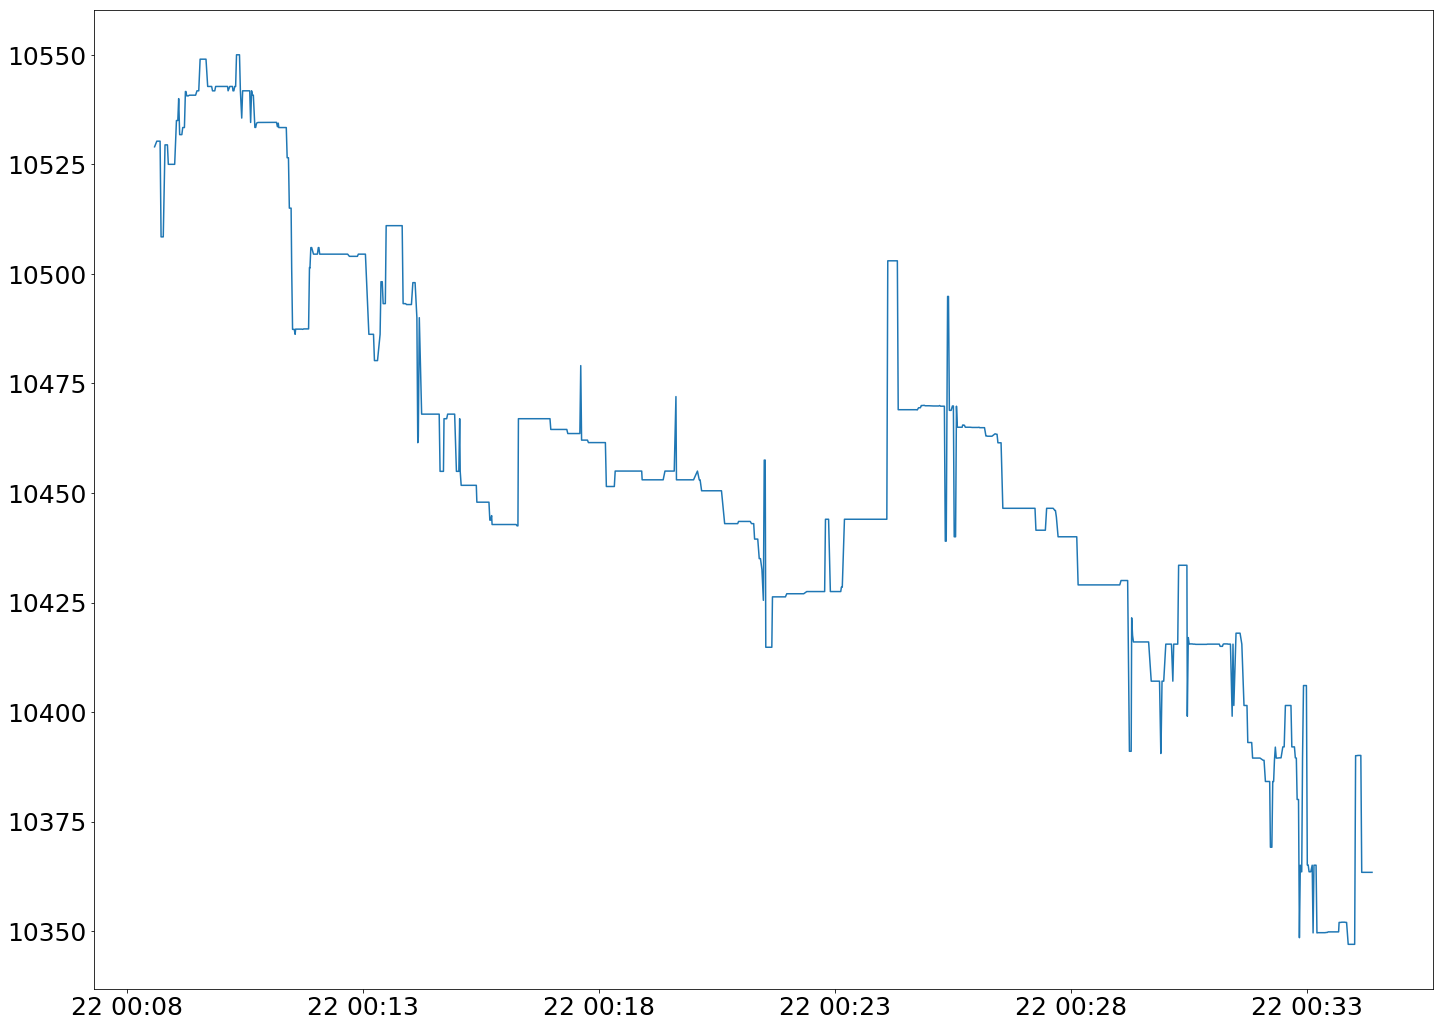
\includegraphics[width=\textwidth]{sample-down-price}
        \caption{30 minute downwards trend}
        \label{fig:sample-down-price}
    \end{subfigure}
    \begin{subfigure}[b]{0.45\textwidth}
        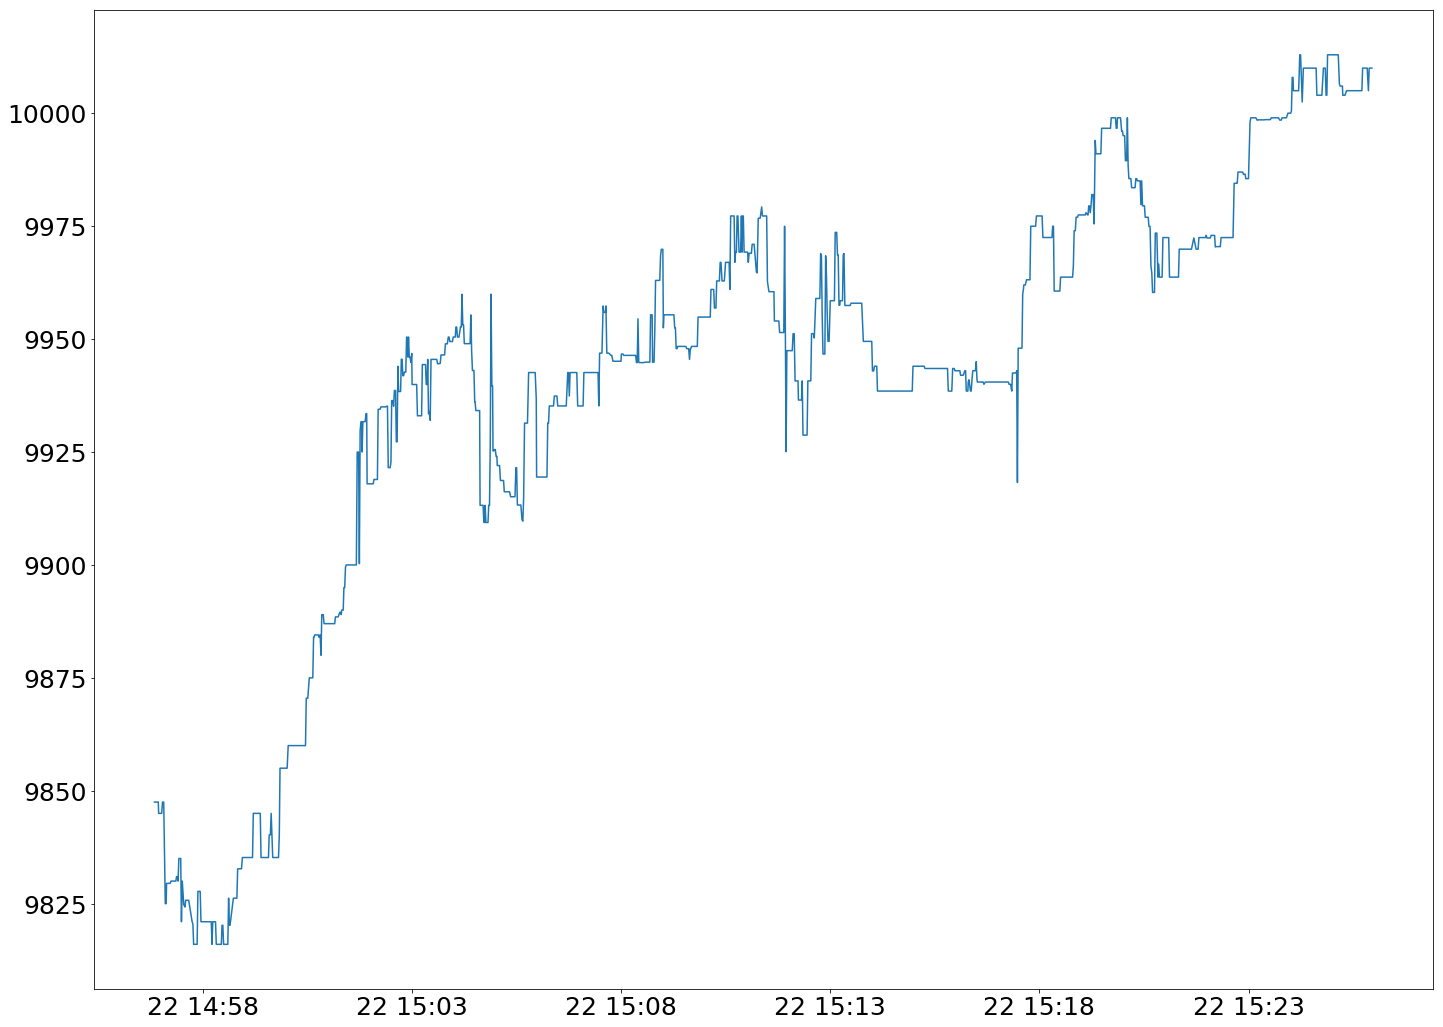
\includegraphics[width=\textwidth]{sample-up-price}
        \caption{30 minute upwards trend}
        \label{fig:sample-up-price}
    \end{subfigure}
    \caption{Bid/ask mid-price of 30 minute order book recordings.}
    \label{fig:sample-price}
\end{figure}
Reasons for choosing two very distinguishable data sets include to determine the ability of the learners to react on a variety of market situations.
As explained in the following section, the expected return of a learner for buying and selling assets heavily depends on the market price movement and therefore the situations become very different for the data sets in use.

When reinforcement learning is applied, the data sets are split with ratio $2:1$, resulting in a training set of $\sim$20 minutes and a test set of $\sim$10 minutes.

\section{An empirical investigation of the reinforcement learning environment}

This section serves to investigate the relationship between the limit order placement and the received reward, for the corresponding orders.
The demonstrated methods are based on the related work described in Section \ref{sec:related-execution-behaviour} and provide the ability to empirically evaluate the reinforcement learning environment (Chapter \ref{chap:setup}) by simulating the behaviour of an agent that buys and sells shares at every possible limit level and records the received rewards (e.g. immediate returns).
The return is denoted by the difference between the market price prior the order placement and the volume weighted average price (VWAP) paid, respectively received, as stated in Eq. \ref{setup:reward}.
As a result we gain understanding of the behaviour of order placement within a given historical market and set a baseline for the reinforcement learners to come.

We recapitulate that according to \cite{nevmyvaka2005electronic, yingsaeree2012algorithmic} there are three obvious trading strategies in order to determine the execution price of an order (considering limit and market order types only):
\begin{enumerate}
    \item Submit a market order tor the entire amount immediately.
    \item Wait until the end of the time period and then go to the market with the entire amount.
    \item Submit a limit order at the beginning of the time period; then submitting a market order for the remainder of shares (if any) at the end of the interval.
\end{enumerate}
Having a total time horizon of 100 seconds available, the last approach is of interested in this analysis.
However, we investigate the behaviour on progressive increasing time horizons, starting from 10 seconds up to 100 seconds, as this demonstrates the discrete time steps to be taken by a learner.
By doing so, the expected return is observed by the average return of placing (e.g. cross-validating) 100 orders of size 1.0 BTC at a random point in the given data set.
The price of the orders are determined by a range of 201 limit levels ($-100...100$) with step size \$0.10, resulting in orders priced in the range of $p_m-10 \ \dots \ p_m+10$, whereas $p_m$ is the market price before the order was placed.

\subsection{Order placement behaviour on data set I}
For the data set I, where the market undergoes a downwards trend, the intuition is as follows:
We expect buy orders to result in better returns when placing deep in the order book, meaning with a highly negative limit level.
Since the price tends to fall, the assumption is that an agent is able to buy for a lower price once time has passed.
Therefore, the longer the time horizon, the lower the limit level can be chosen in order to still be able to execute the full amount of shares.
Contrarily, we expect sell orders to provide better returns when the agent crosses the spread with a positive limit level.
The assumption is that in a falling market it is unlikely that market participants are willing to buy for higher prices and therefore the agent must place sell orders higher in the book in order to sell immediately.
Otherwise, the longer the time horizon, the less return an agent would retrieve as the market order after the order has not been filled becomes costly.
We proceed this investigation within our reinforcement learning environment as shown Figure \ref{fig:behvaiour-down}.
Therefore, time horizons of 10, 30, 60 and 100 seconds (y-axis) and limit levels reaching from -100 to +100 (x-axis) were chosen.
The time horizons determine the various situations an agent is confronted while proceeding steps within an epoch.
The limit levels are chosen broadly in order to retrieve understanding about the outcome of a variety of possible actions.

With a time horizon of only 10 seconds left, the expected behaviour is, however, proven wrong.
For buy orders, shown in Figure \ref{fig:behvaiour-down-10s-buy}, the returns suggest to place the orders close to the spread, but still on the opposing side, at a limit level of $\sim$+5.
The spike at limit level $\sim$-5 indicates that the overall best return was provided at this level, however it comes with the risk that the orders fails to execute, indicated by the downwards spike also close to level $\sim$-5.
For selling within 10 seconds, as shown in Figure \ref{fig:behvaiour-up-10s-sell}, the best return is given when crossing the spread with a positive limit level of $\sim$+50.
The spike at limit level $\sim$-70 is likely caused by one of the orders during the cross-validation process, that was able to execute and therefore contributed to greater return.

With an increased time horizon of a total of 30 seconds, as shown in Figures \ref{fig:behvaiour-down-30s-buy} and \ref{fig:behvaiour-down-30s-sell}, the expected behaviour becomes more evident.
Positive returns can be achieved by posting buy orders deep in the order book, whereas there is not much variance between the negative limit levels itself.
Therefore, we can expect that in the given market situation the agent was able to execute the order partially at very low limit levels and for the unexecuted part a market order followed which ultimately averaged the price to be similar as when the agent placed the order initially at a price which is only slightly below the spread.
This is confirmed by the fact that the most dense range of positive returns is indeed around the limit levels just below the spread.
Crossing the spread causes increasingly lower returns, the more positive the limit level is chosen.
That is a result of agents willingness to immediately buy for an increasing price by using market orders.
The opposite effect occurs while selling assets.
Market orders higher in the book result in result in better returns than limit orders deep in the book.
Interestingly, orders which were placed very deep in the book, at limit level $\sim$-50 and below, are rewarded better than the ones close to the spread.
This is most likely a consequence of a minority of orders which were partially filled at this level during the cross-validation process.

With time horizons of 60 and 100 seconds the expected behaviour of the orders is clearly given.
Buy orders as shown in Figures \ref{fig:behvaiour-down-60s-buy} and \ref{fig:behvaiour-down-100s-buy}, best best off when placed very deep in the order book.
However, when placed too deep, at level -100, the return is slightly less as a result of unexecuted orders which had to be filled with market orders once the time was consumed.
In addition, positive limit levels become stable since there are more sellers in the market with the extended time horizon and therefore very high placed orders have the same effect as limit orders posted only slightly above the spread.
The same applies to sell orders which are placed very deep in the book, as shown in Figures \ref{fig:behvaiour-up-60s-sell} and \ref{fig:behvaiour-up-100s-sell}.
Placing orders very deep in the book have the same effect as when placing the order just below the spread, that is, there are no traders willing to buy at such a high price and therefore market orders follow once the time has passed.
\vfill
\newpage
\begin{figure}[H]
    \centering
    \begin{subfigure}[b]{0.45\textwidth}
        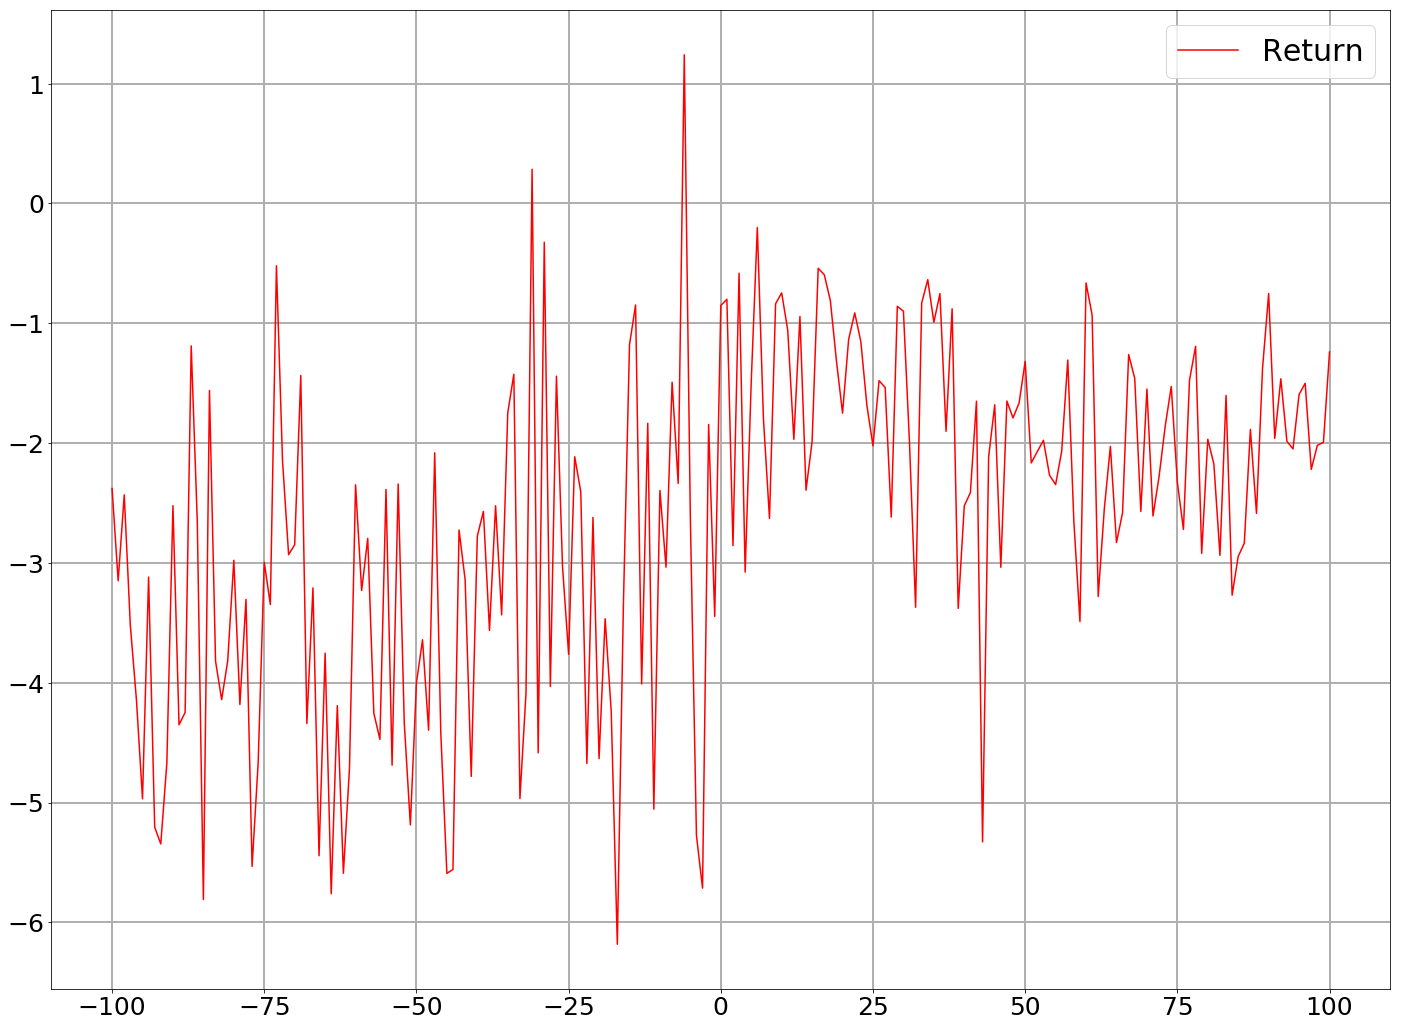
\includegraphics[width=\textwidth]{images/behaviour-10s-buy.png}
        \caption{Returns of buy orders within 10 seconds}
        \label{fig:behvaiour-down-10s-buy}
    \end{subfigure}
    \begin{subfigure}[b]{0.45\textwidth}
        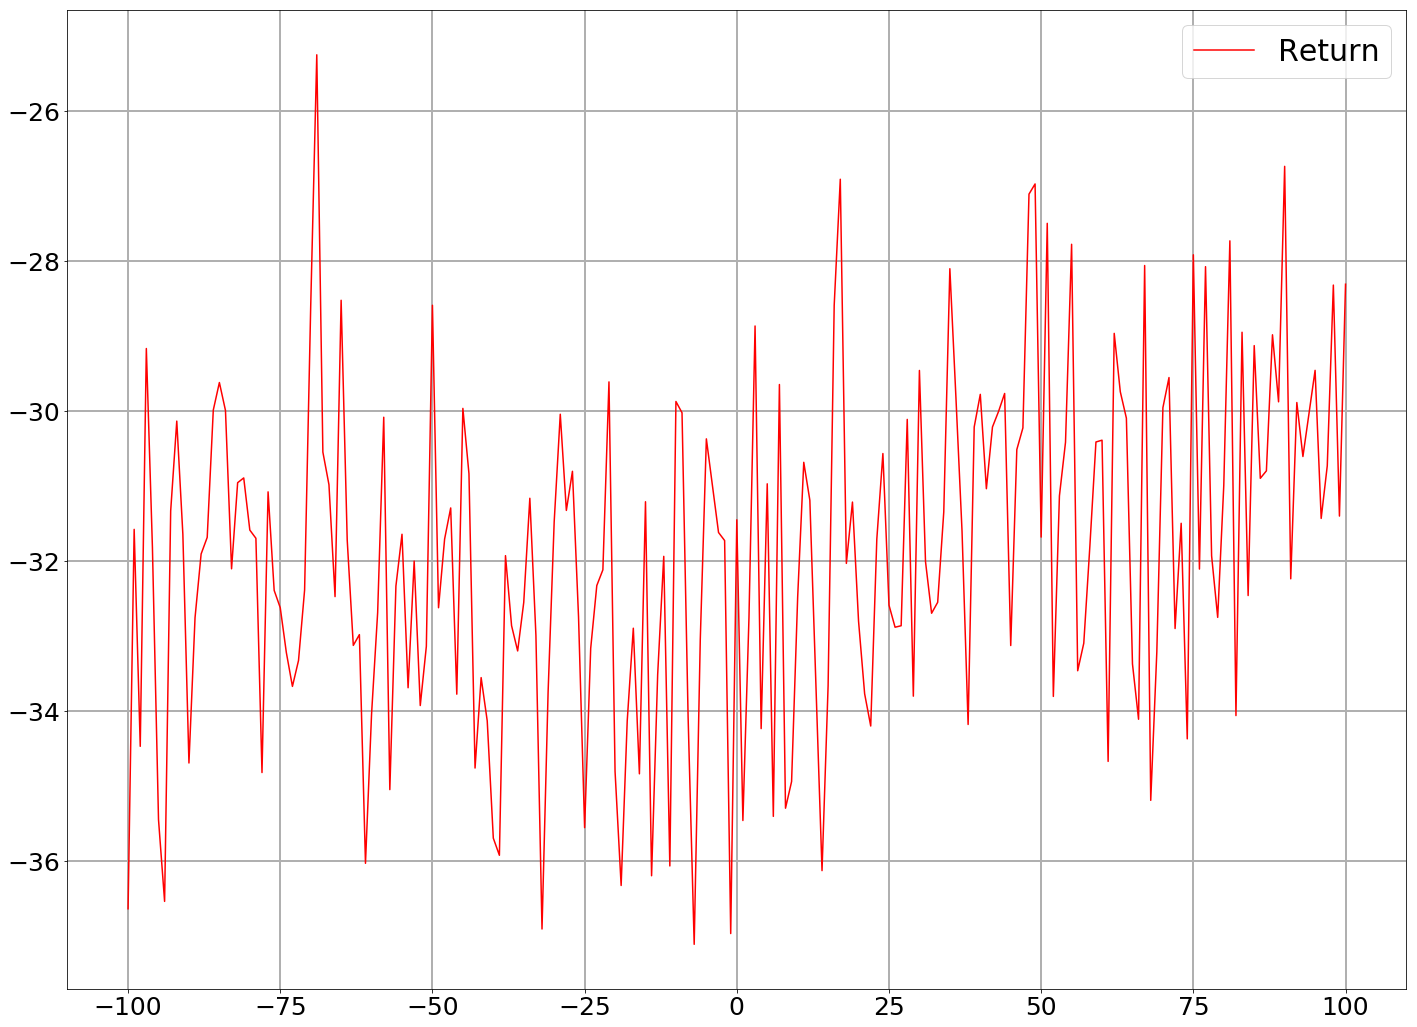
\includegraphics[width=\textwidth]{images/behaviour-10s-sell.png}
        \caption{Returns of sell orders within 10 seconds}
        \label{fig:behvaiour-down-10s-sell}
    \end{subfigure}
    \begin{subfigure}[b]{0.45\textwidth}
        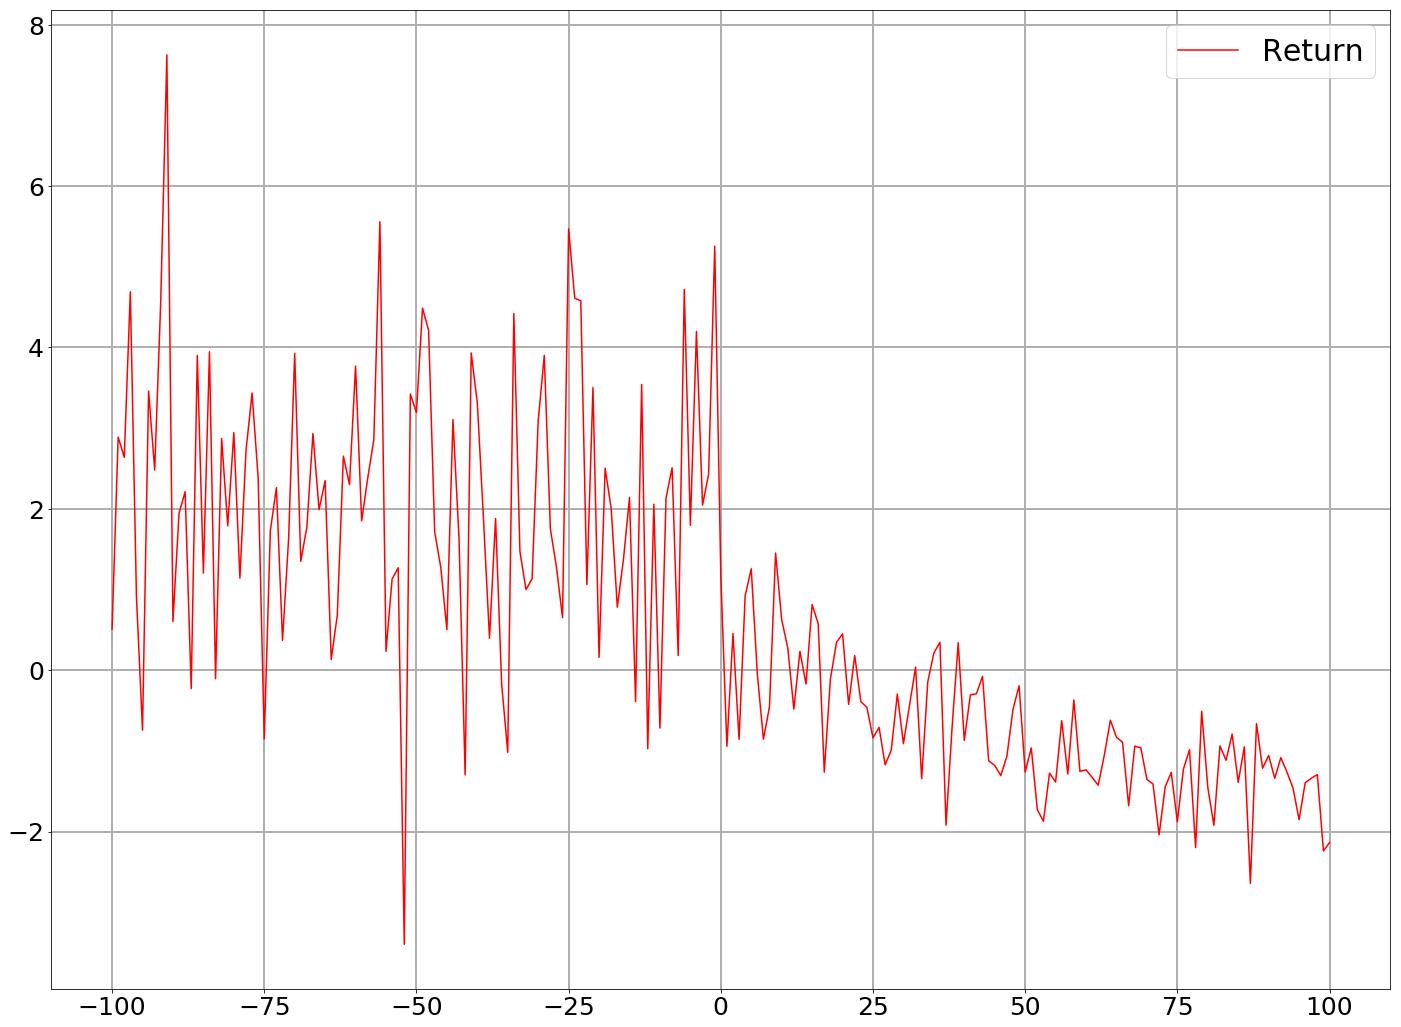
\includegraphics[width=\textwidth]{images/behaviour-30s-buy.png}
        \caption{Returns of buy orders within 30 seconds}
        \label{fig:behvaiour-down-30s-buy}
    \end{subfigure}
    \begin{subfigure}[b]{0.45\textwidth}
        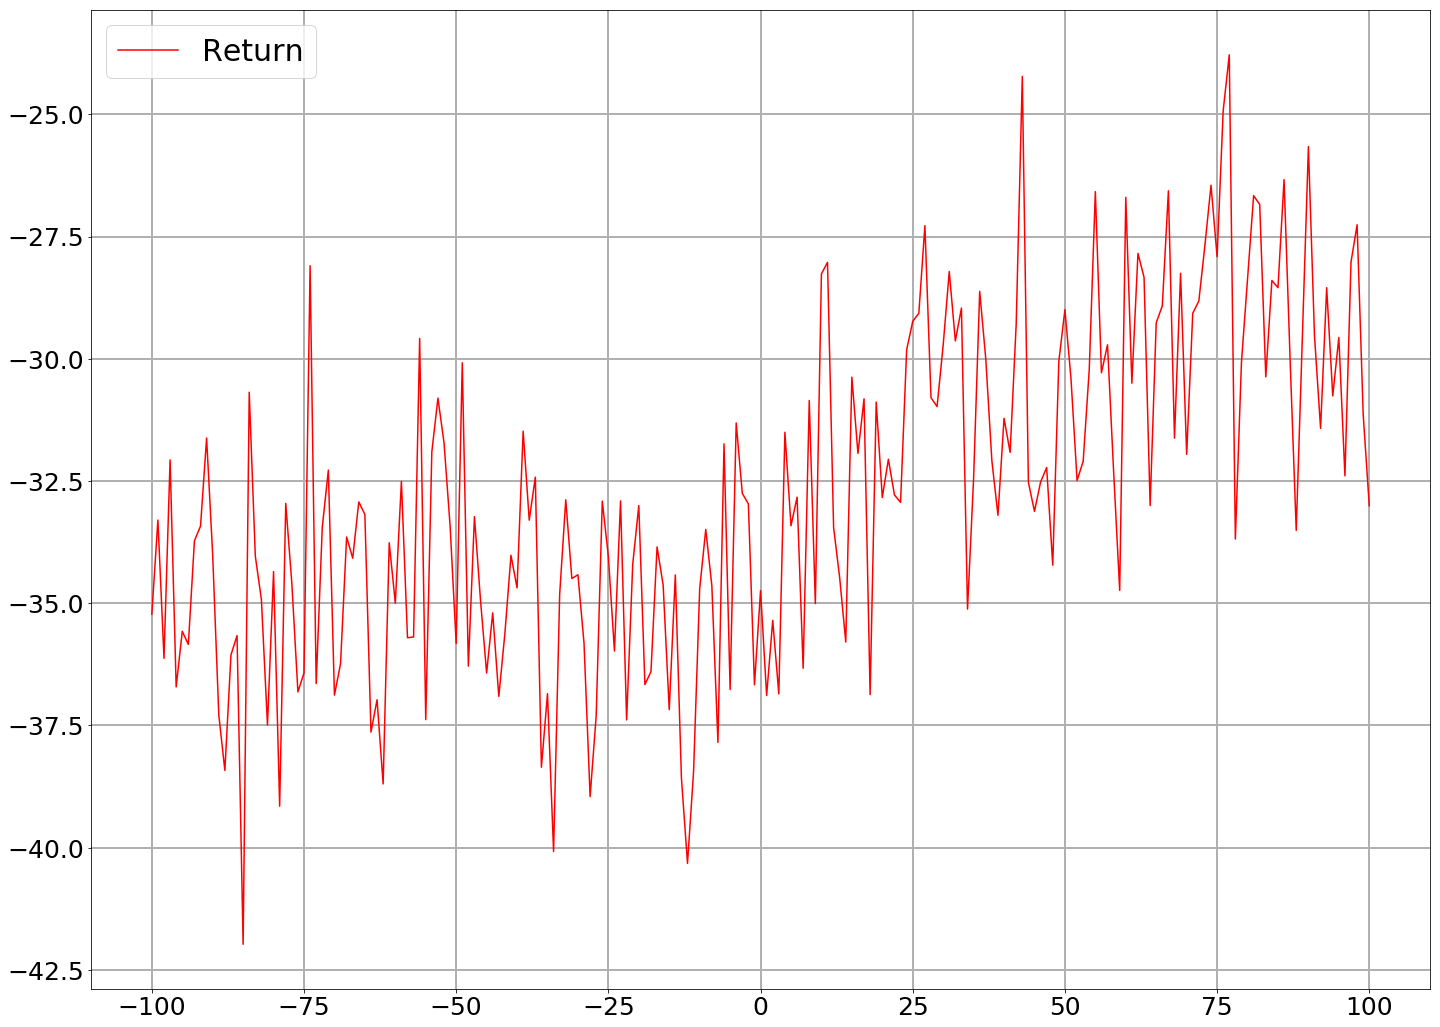
\includegraphics[width=\textwidth]{images/behaviour-30s-sell.png}
        \caption{Returns of sell orders within 30 seconds}
        \label{fig:behvaiour-down-30s-sell}
    \end{subfigure}
    \begin{subfigure}[b]{0.45\textwidth}
        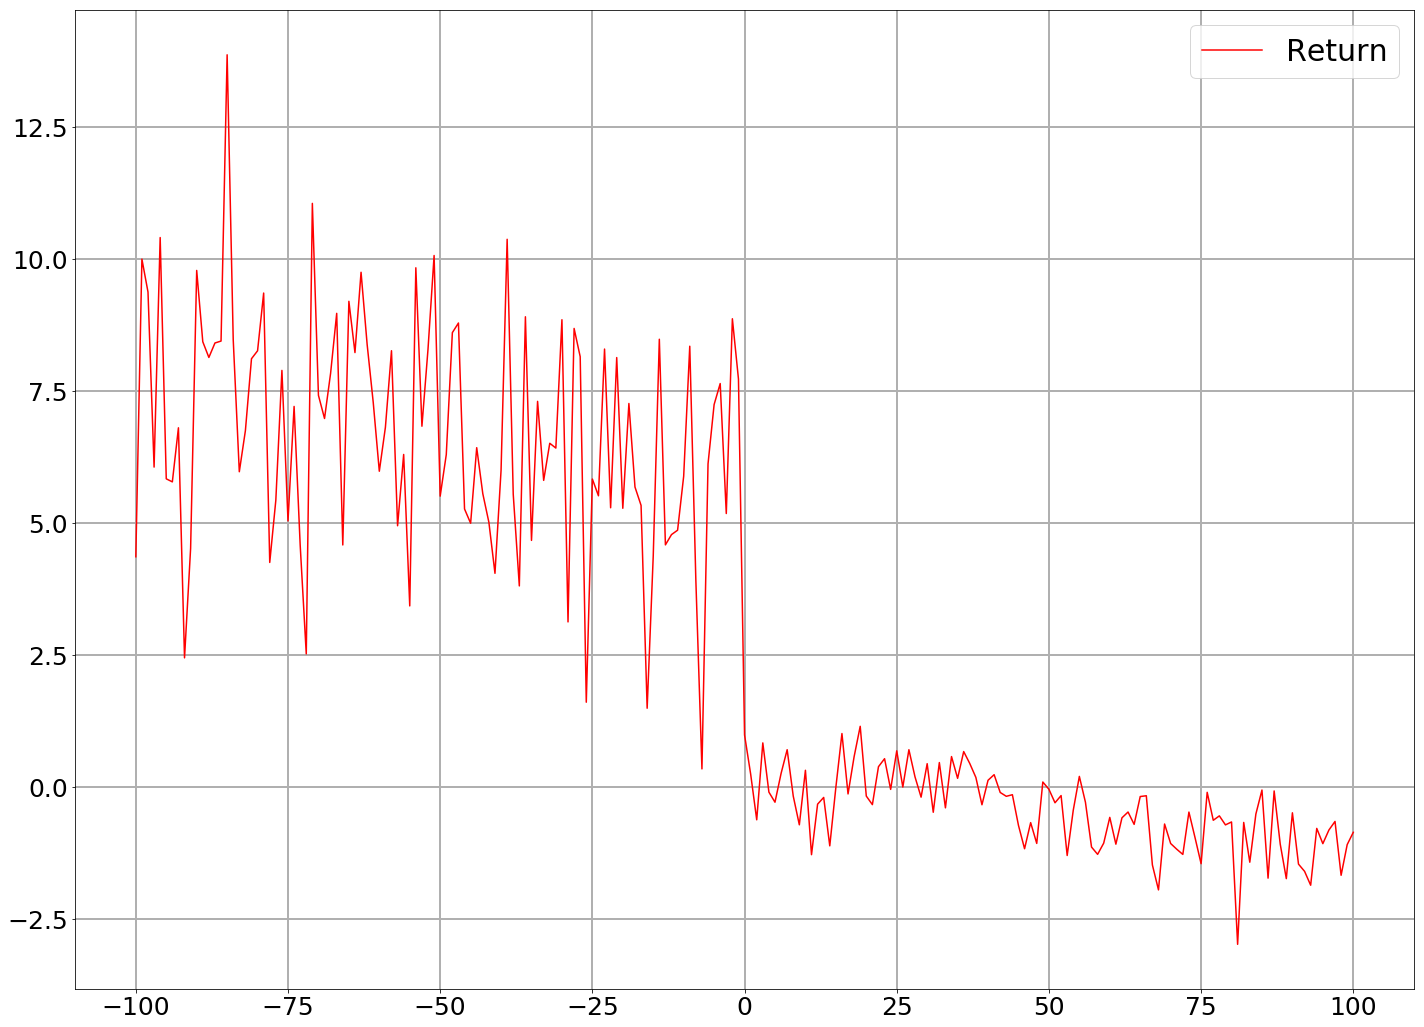
\includegraphics[width=\textwidth]{images/behaviour-60s-buy.png}
        \caption{Returns of buy orders within 60 seconds}
        \label{fig:behvaiour-down-60s-buy}
    \end{subfigure}
    \begin{subfigure}[b]{0.45\textwidth}
        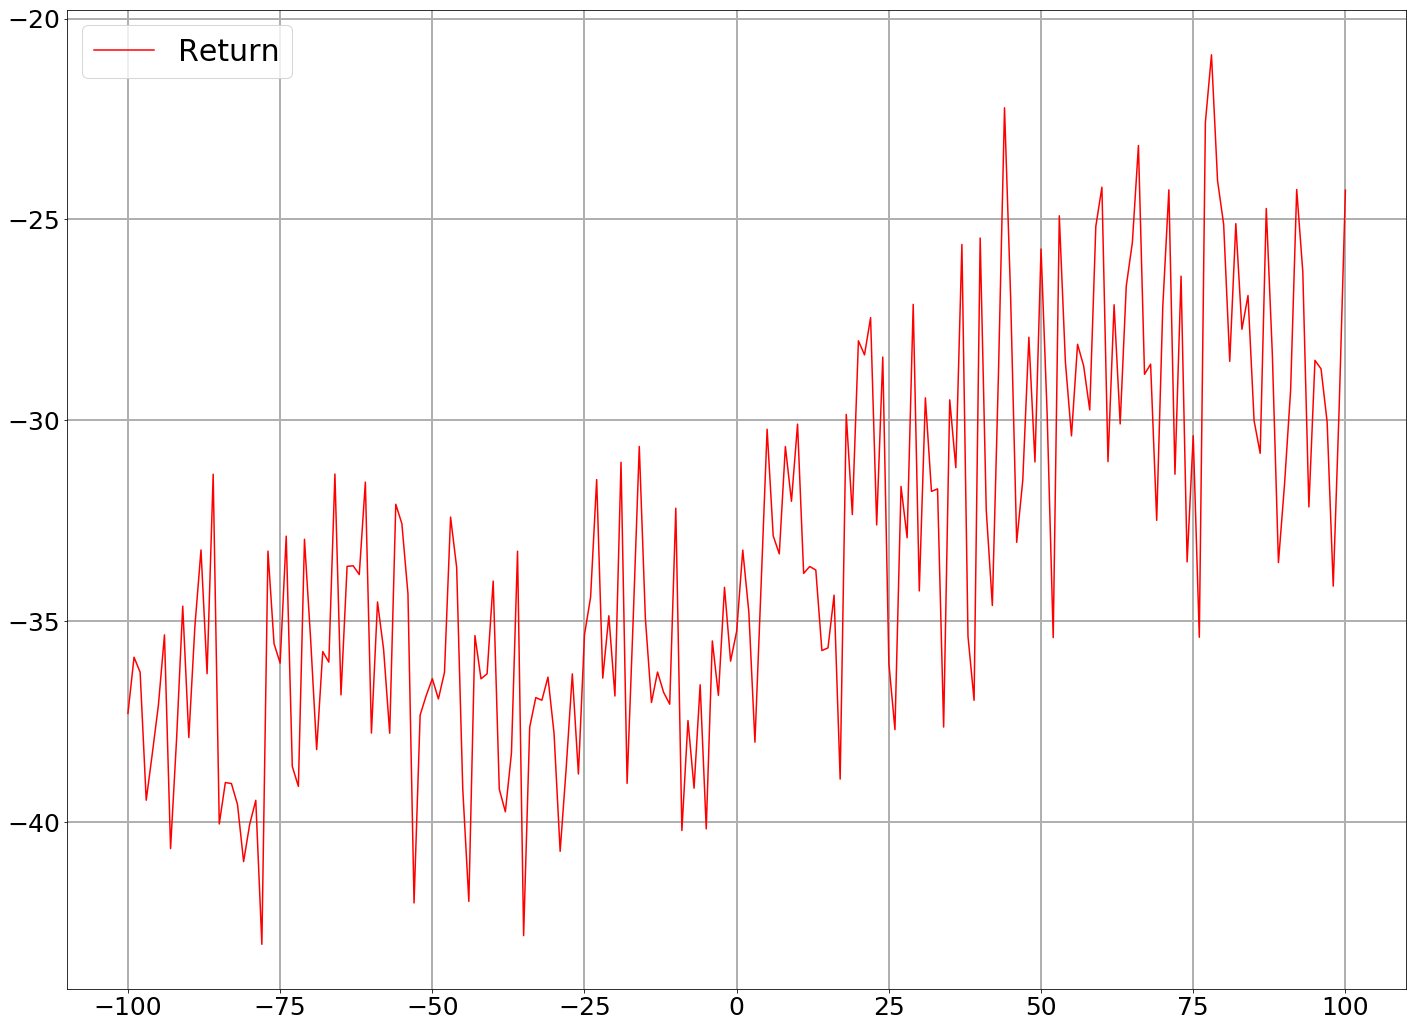
\includegraphics[width=\textwidth]{images/behaviour-60s-sell.png}
        \caption{Returns of sell orders 60 seconds}
        \label{fig:behvaiour-down-60s-sell}
    \end{subfigure}
    \begin{subfigure}[b]{0.45\textwidth}
        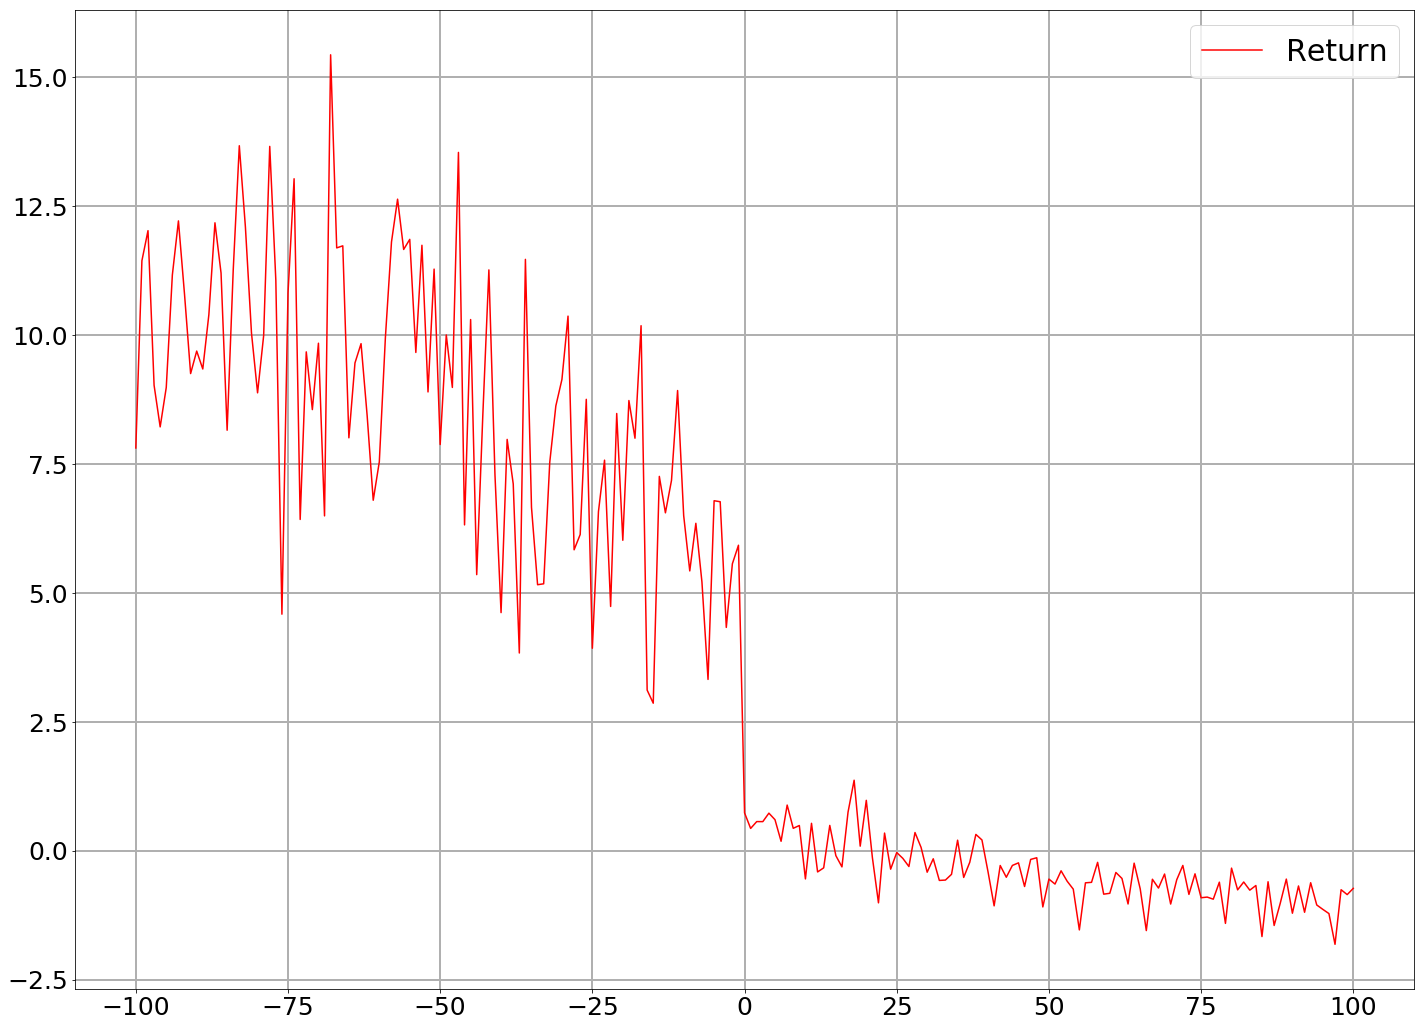
\includegraphics[width=\textwidth]{images/behaviour-100s-buy.png}
        \caption{Returns of buy orders 100 seconds}
        \label{fig:behvaiour-down-100s-buy}
    \end{subfigure}
    \begin{subfigure}[b]{0.45\textwidth}
        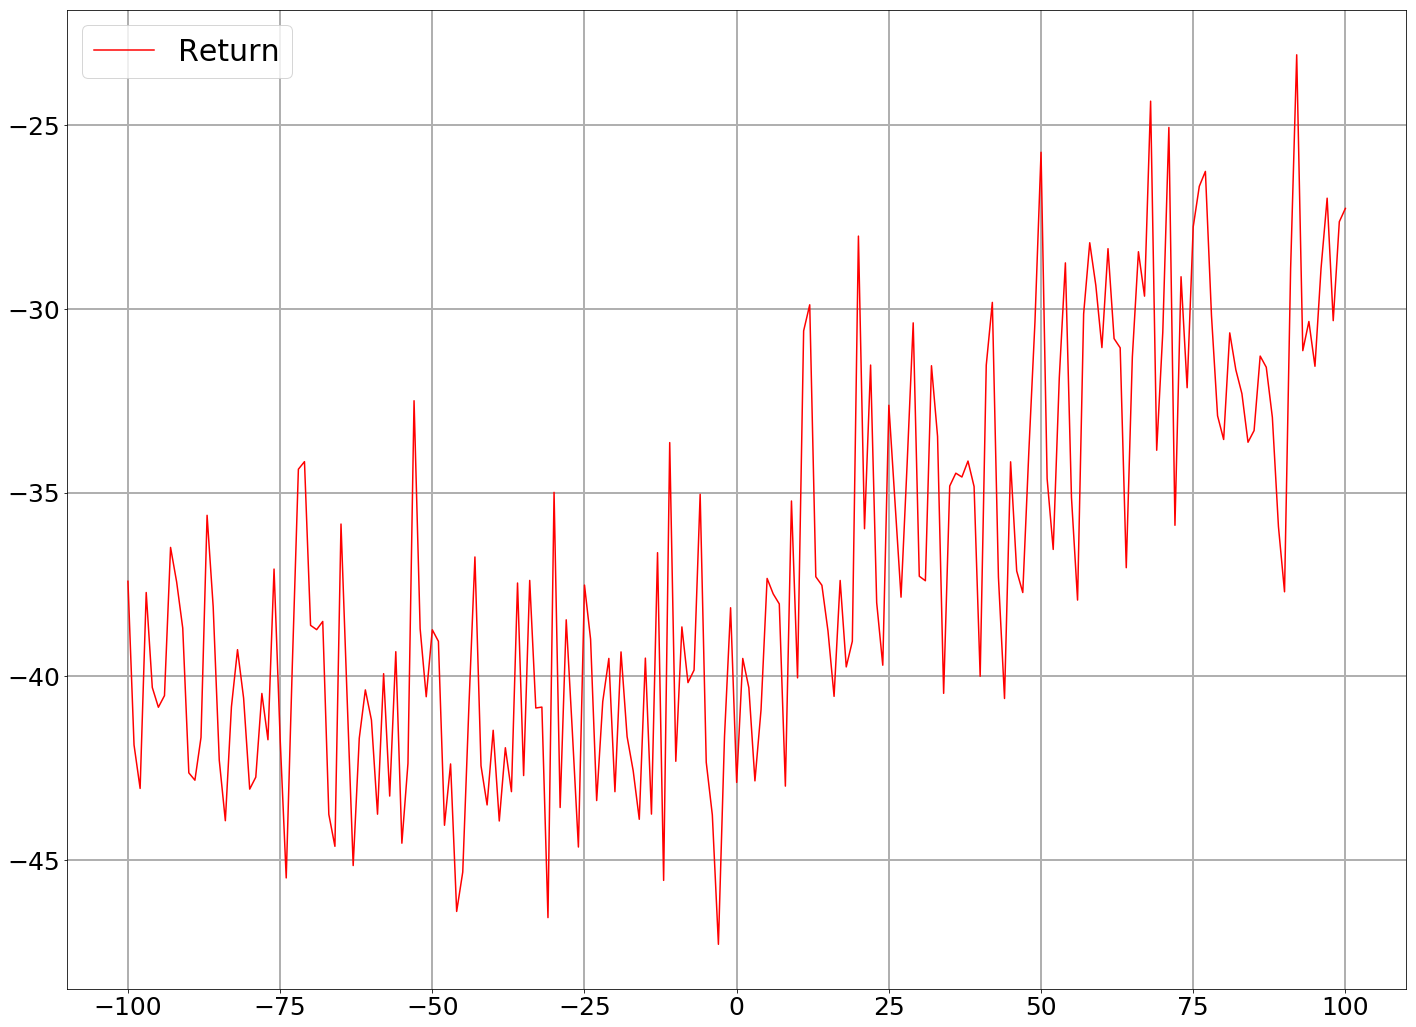
\includegraphics[width=\textwidth]{images/behaviour-100s-sell.png}
        \caption{Returns of sell orders 100 seconds}
        \label{fig:behvaiour-down-100s-sell}
    \end{subfigure}
    \caption{Returns of buy and sell orders executed within 10, 30, 60 and 100 seconds on data set I.}
    \label{fig:behvaiour-down}
\end{figure}

\subsection{Order placement behaviour on data set II}
For the data set II, which contains an upwards trend, the intuition is the opposite as during the investigation of data set I.
Namely, we expect buy orders to result in better returns when immediately filled, that is when the agent crosses the spread and places the order high in the book.
The assumption is that as time passes and the market price rises, other traders become less willing to sell for the market price or lower.
Therefore, the longer the time horizon given to the agent, the more critical it becomes to execute immediately, as otherwise shares would have to be bought to an increased market price.
Likewise, better returns of sell orders are expected when placed deep in the book, meaning to be sold at a higher price.
The assumption is that as the price rises, market participants become more likely to buy assets for higher prices.
Hence, the longer the time horizon, the deeper the agent should place a limit sell order in the book, as this will likely not require a following market order due to (partially) unexecuted shares.
We investigate these assumptions by proceeding the same experiment as in the previous section, as shown in Figure \ref{fig:behvaiour-up}, whereas time horizons of 10, 30, 60 and 100 seconds (y-axis) and limit levels reaching from -100 to +100 (x-axis) were chosen

The returns of buy orders with a time horizon of 10 seconds, as shown in Figure \ref{fig:behvaiour-up-10s-buy}, correlate with the above stated assumptions.
That is, highest returns are achieved when crossing the spread and although limit levels in the range of 1-50 tend to perform the same, the wises choice for the agent would be to choose the one closest to the spread as it comes with the least risk of paying a premium.
With the same time horizon, the sell orders placed contradict the assumptions, as shown in Figure \ref{fig:behvaiour-up-10s-sell}.
Here the agent is rewarded the most when choosing a price for the order at market price, as indicated by the limit level 0, that is on the spread.
A highly negative limit level causes to receive approximately \$3.00 less than when placing at the suggested market price.

With 30 seconds left to buy 1.0 BTC, in Figure \ref{fig:behvaiour-up-30s-buy}, the orders placed above the spread become stable for any such limit level, much more so than in the previous investigation with the data set I.
This is likely due to the higher order pressure of the data set II, as described in Section \ref{sec:analysis-data-sets}.
Hence, there are more market participants willing to sell.
The return curve that indicates sell orders placed by an agent, shown in Figure \ref{fig:behvaiour-up-30s-sell}, shifts towards a more evenly distributed returns compare to when only 10 seconds were left.
Therefore, limit orders tend to become more rewarding and an agent might benefit from a slight increase in price within the given time horizon.

Even more so, this pattern becomes evident when a time horizon of 60 and 100 seconds were given, as shown in Figures \ref{fig:behvaiour-up-60s-sell} and \ref{fig:behvaiour-up-100s-sell} respectively.
With the increased time horizon the assumptions stated in the beginning of this section are confirmed by shown that the agent, when trying to sell shares, should place orders indeed deep in the order book.
When time passes and the market price rises, market participants are willing to buy for an increasing price and an agent is able to sell all assets for such an increased price without the need of a following market order.
Contrarily, if the agent decides to offer to sell the assets for a decreasing price, as indicated by the higher limit levels above the spread, the less reward would be given.
More precisely, for a time horizon of 100 seconds, the agent would receive up to \$7.00 less when choosing to cross the spread with a limit level of +100 compared to some negative limit level.
Figures \ref{fig:behvaiour-up-60s-buy} and \ref{fig:behvaiour-up-100s-buy} which show the result of an agent that tries to buy assets within the increased time horizon, the behaviour is clear.
That is, during an uprising market, the damage can be minimized by crossing the spread and buying immediately.
The advice stated before remains, that is, the agent should choose a price a few steps (\$0.10) above the market price as there is enough liquidity in the market to buy the demanded number of assets.
\vfill
\newpage
\begin{figure}[H]
    \centering
    \begin{subfigure}[b]{0.45\textwidth}
        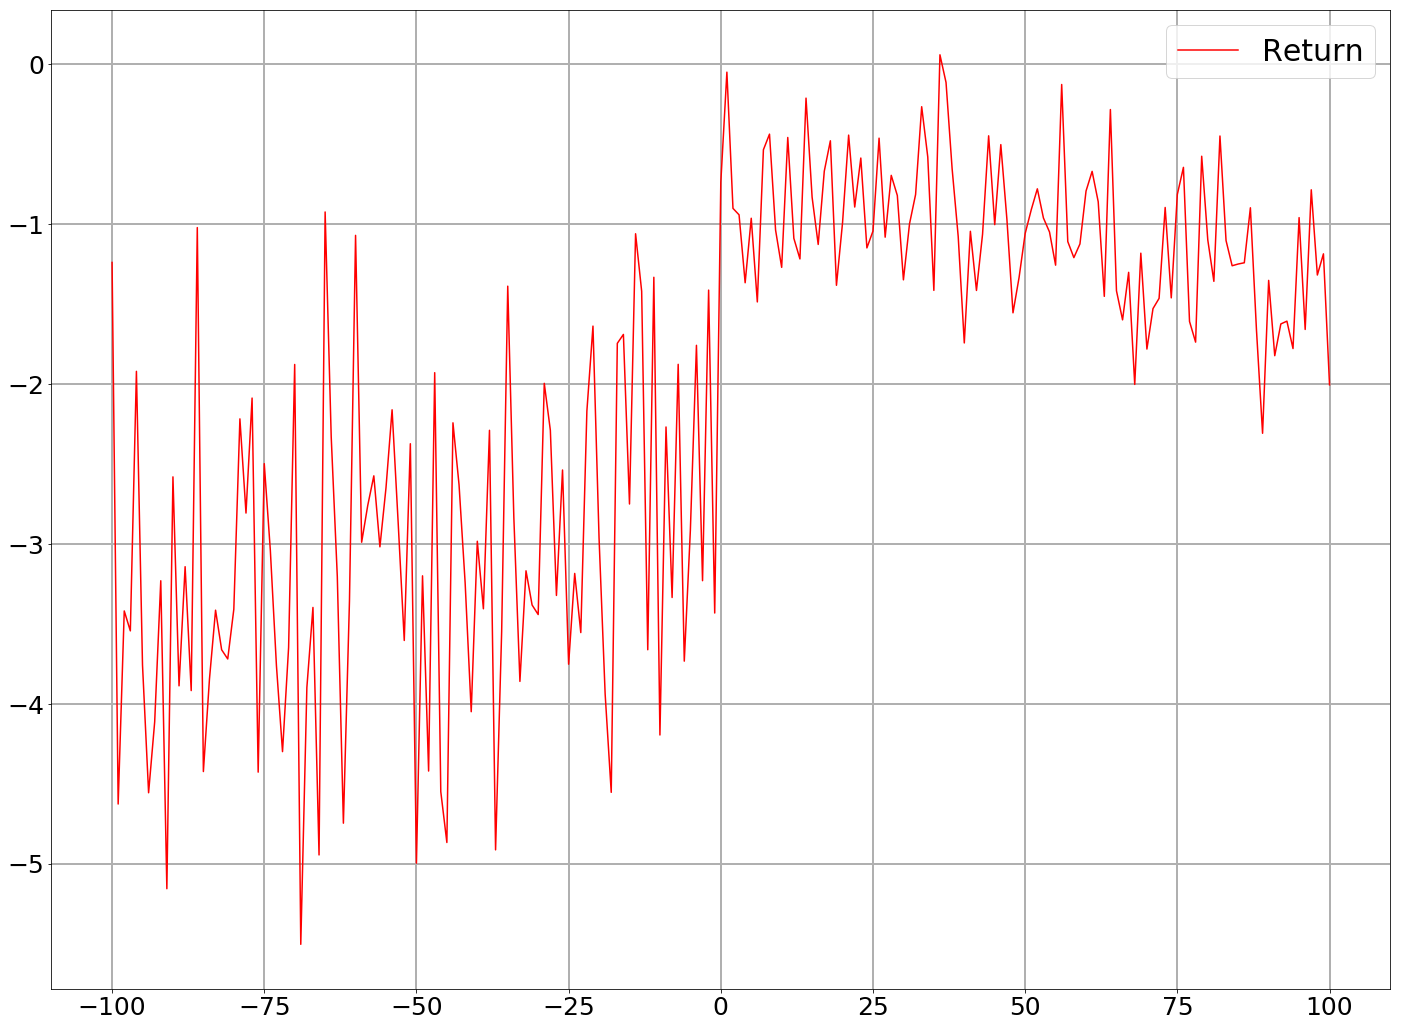
\includegraphics[width=\textwidth]{images/behaviour-up-10s-buy.png}
        \caption{Returns of buy orders within 10 seconds}
        \label{fig:behvaiour-up-10s-buy}
    \end{subfigure}
    \begin{subfigure}[b]{0.45\textwidth}
        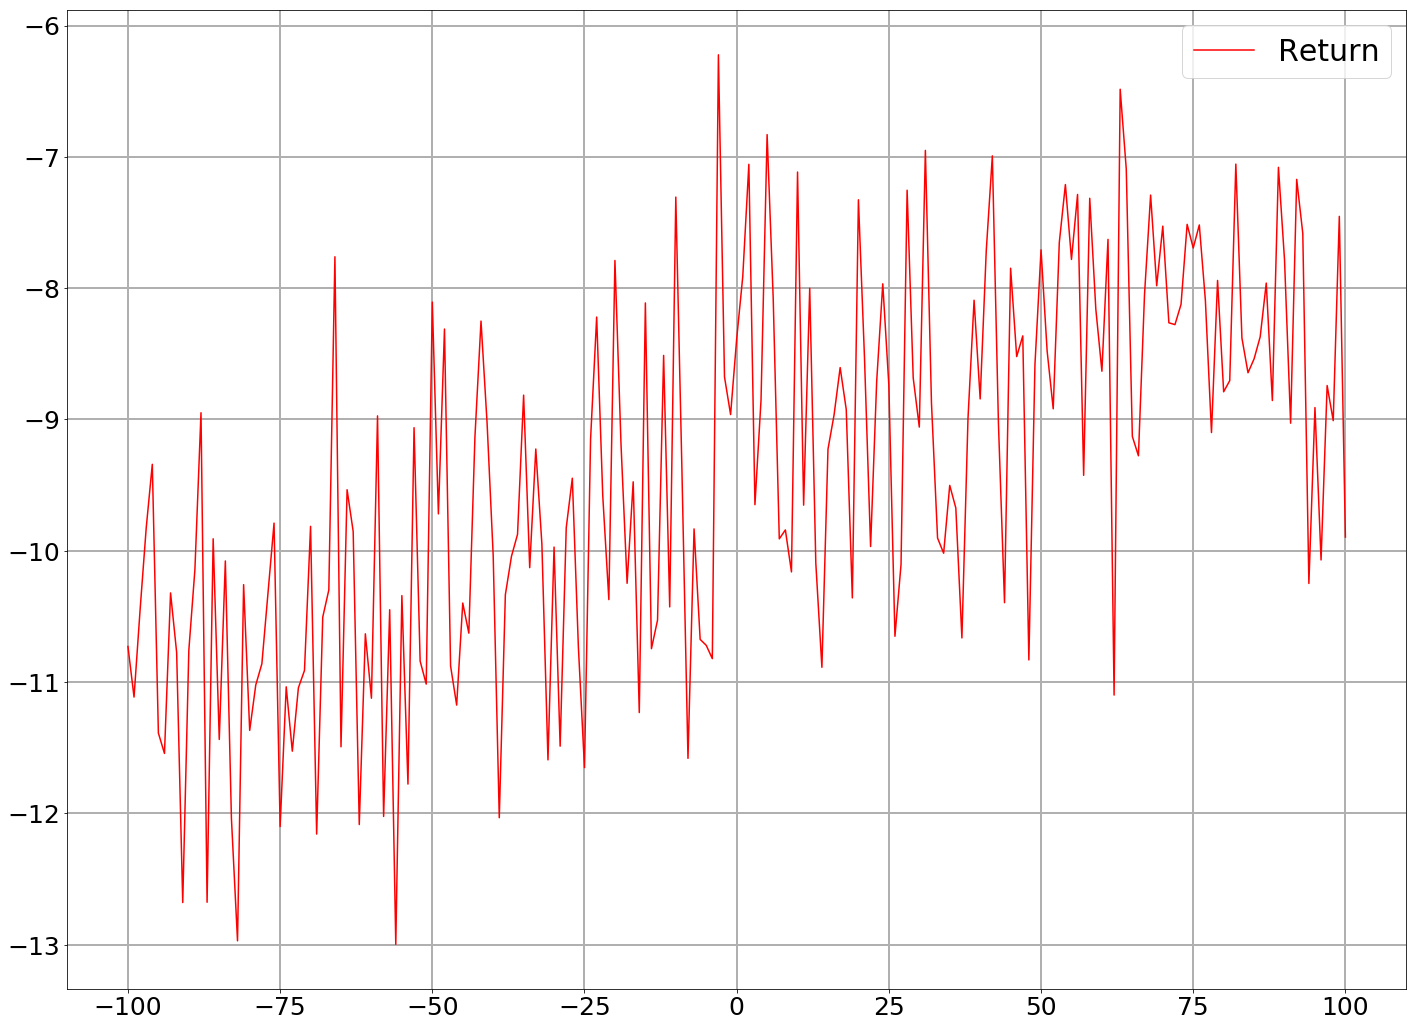
\includegraphics[width=\textwidth]{images/behaviour-up-10s-sell.png}
        \caption{Returns of sell orders within 10 seconds}
        \label{fig:behvaiour-up-10s-sell}
    \end{subfigure}
    \begin{subfigure}[b]{0.45\textwidth}
        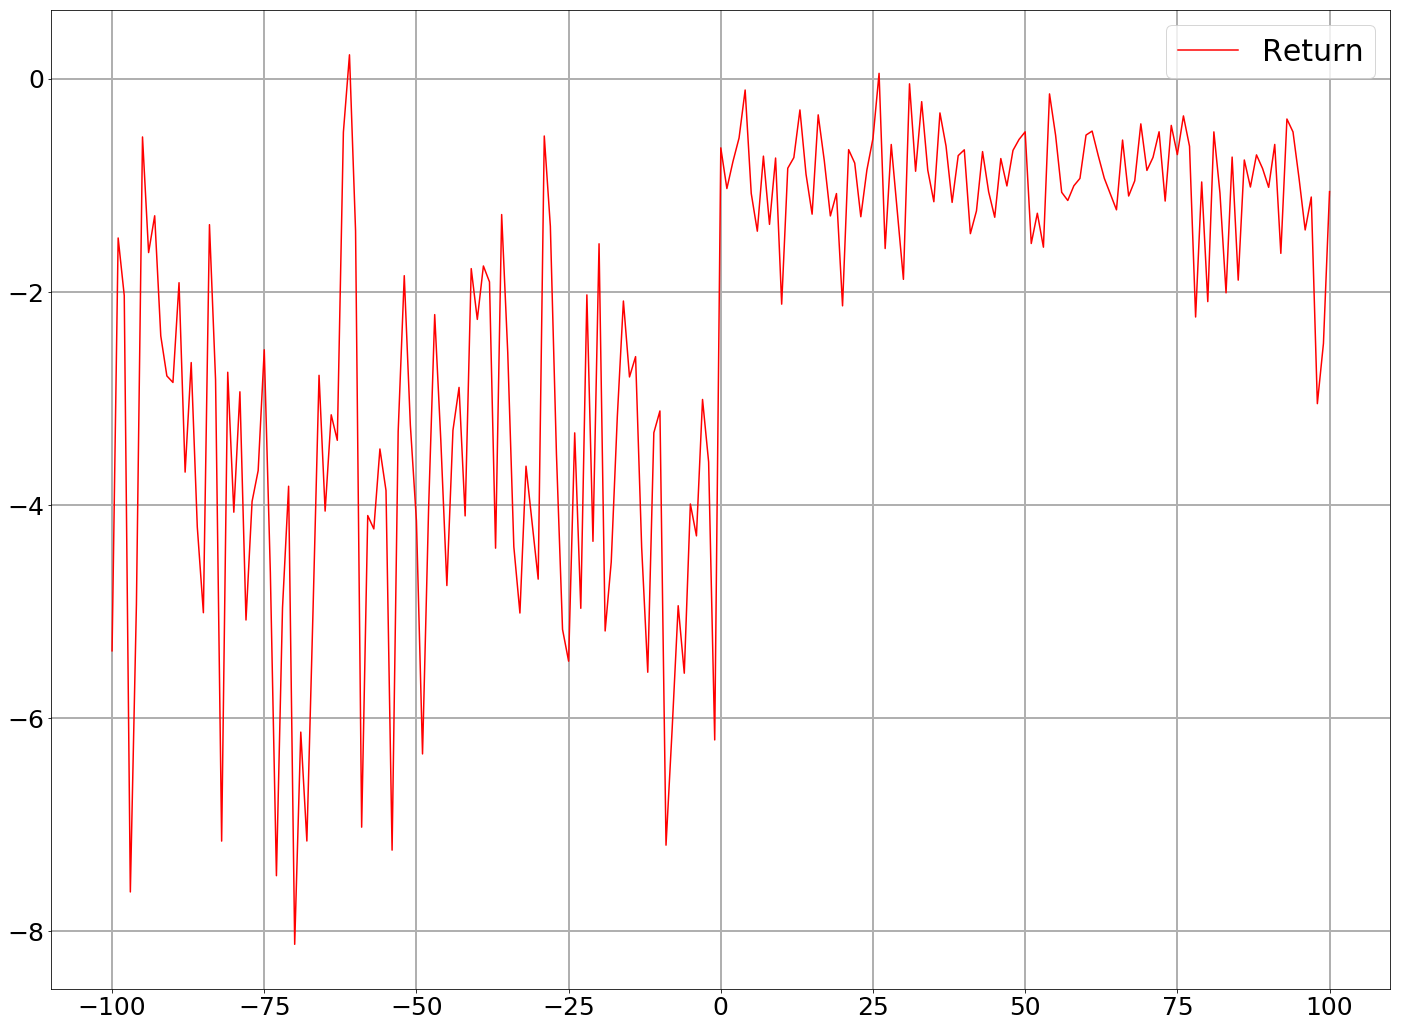
\includegraphics[width=\textwidth]{images/behaviour-up-30s-buy.png}
        \caption{Returns of buy orders within 30 seconds}
        \label{fig:behvaiour-up-30s-buy}
    \end{subfigure}
    \begin{subfigure}[b]{0.45\textwidth}
        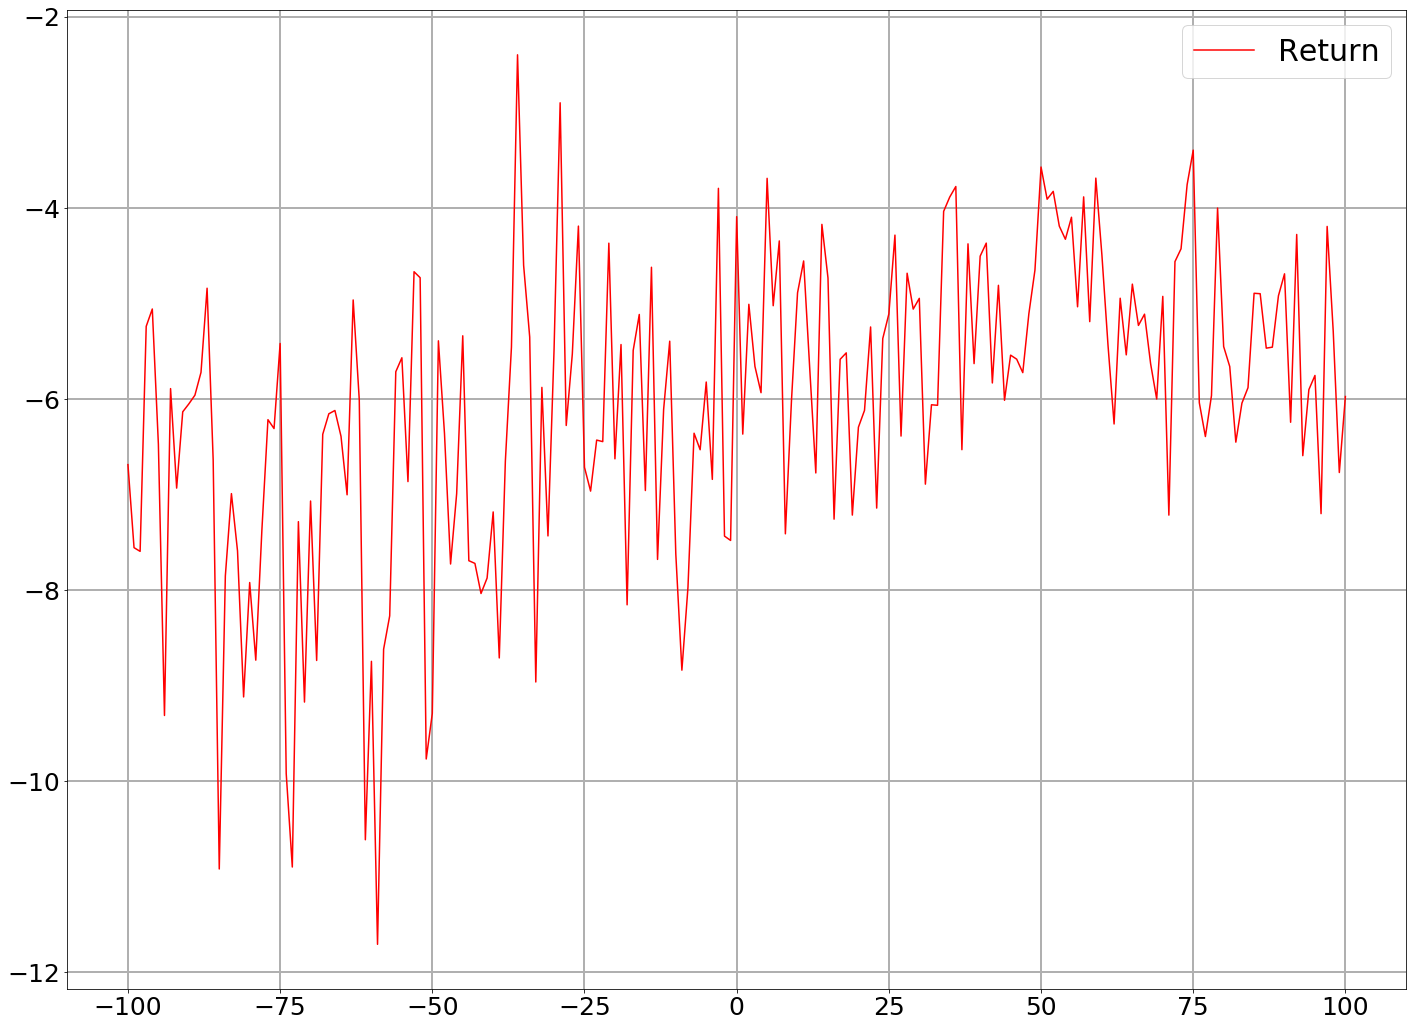
\includegraphics[width=\textwidth]{images/behaviour-up-30s-sell.png}
        \caption{Returns of sell orders within 30 seconds}
        \label{fig:behvaiour-up-30s-sell}
    \end{subfigure}
    \begin{subfigure}[b]{0.45\textwidth}
        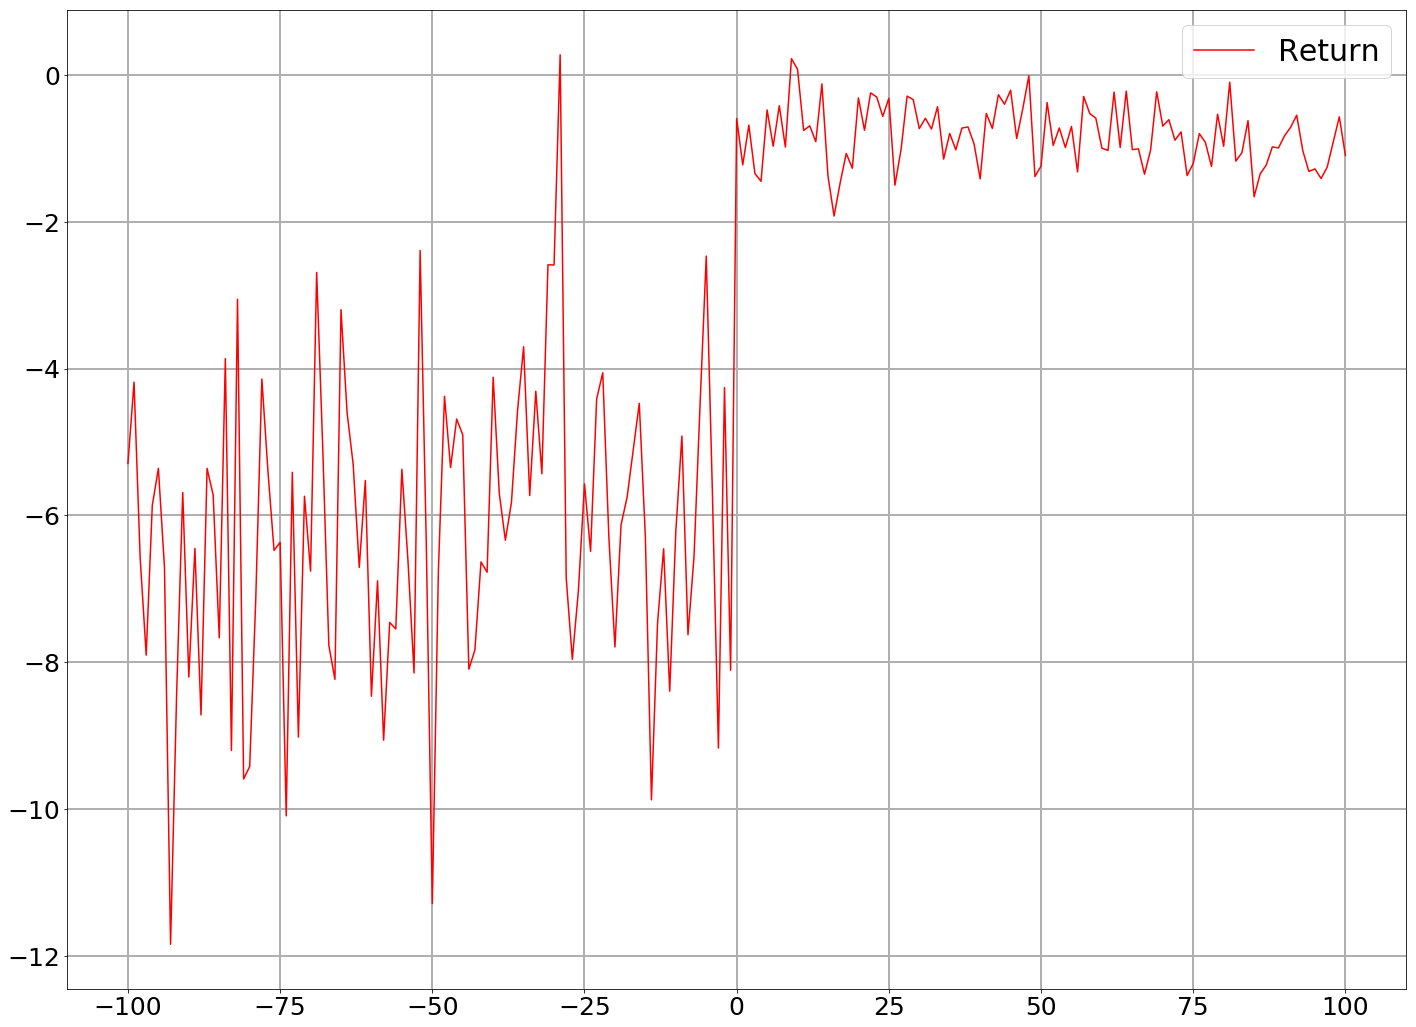
\includegraphics[width=\textwidth]{images/behaviour-up-60s-buy.png}
        \caption{Returns of buy orders within 60 seconds}
        \label{fig:behvaiour-up-60s-buy}
    \end{subfigure}
    \begin{subfigure}[b]{0.45\textwidth}
        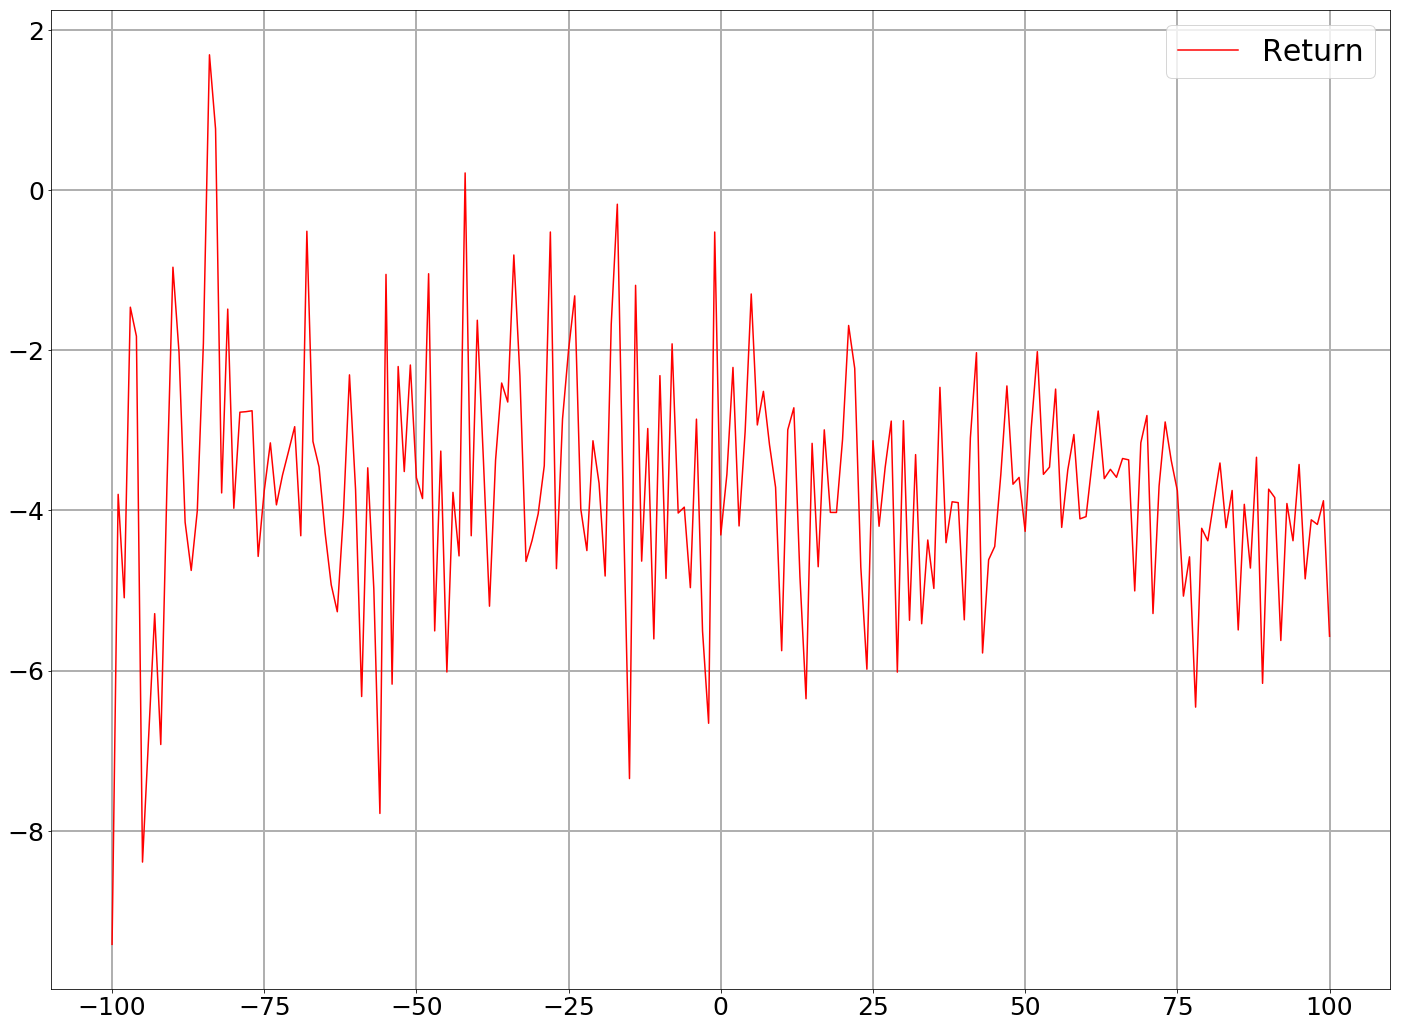
\includegraphics[width=\textwidth]{images/behaviour-up-60s-sell.png}
        \caption{Returns of sell orders 60 seconds}
        \label{fig:behvaiour-up-60s-sell}
    \end{subfigure}
    \begin{subfigure}[b]{0.45\textwidth}
        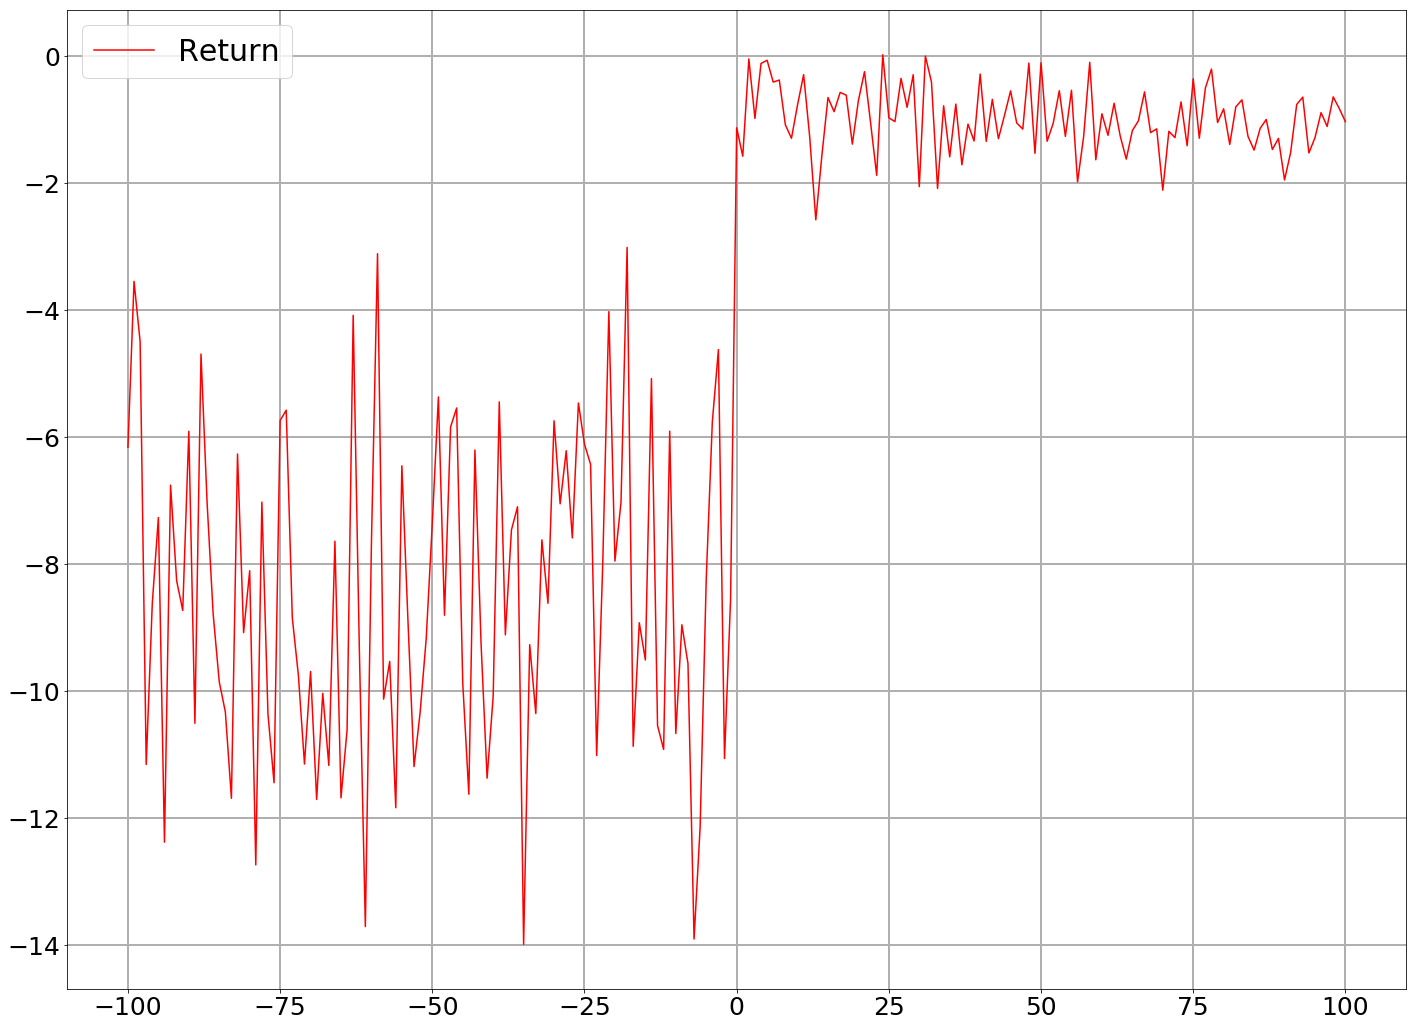
\includegraphics[width=\textwidth]{images/behaviour-up-100s-buy.png}
        \caption{Returns of buy orders 100 seconds}
        \label{fig:behvaiour-up-100s-buy}
    \end{subfigure}
    \begin{subfigure}[b]{0.45\textwidth}
        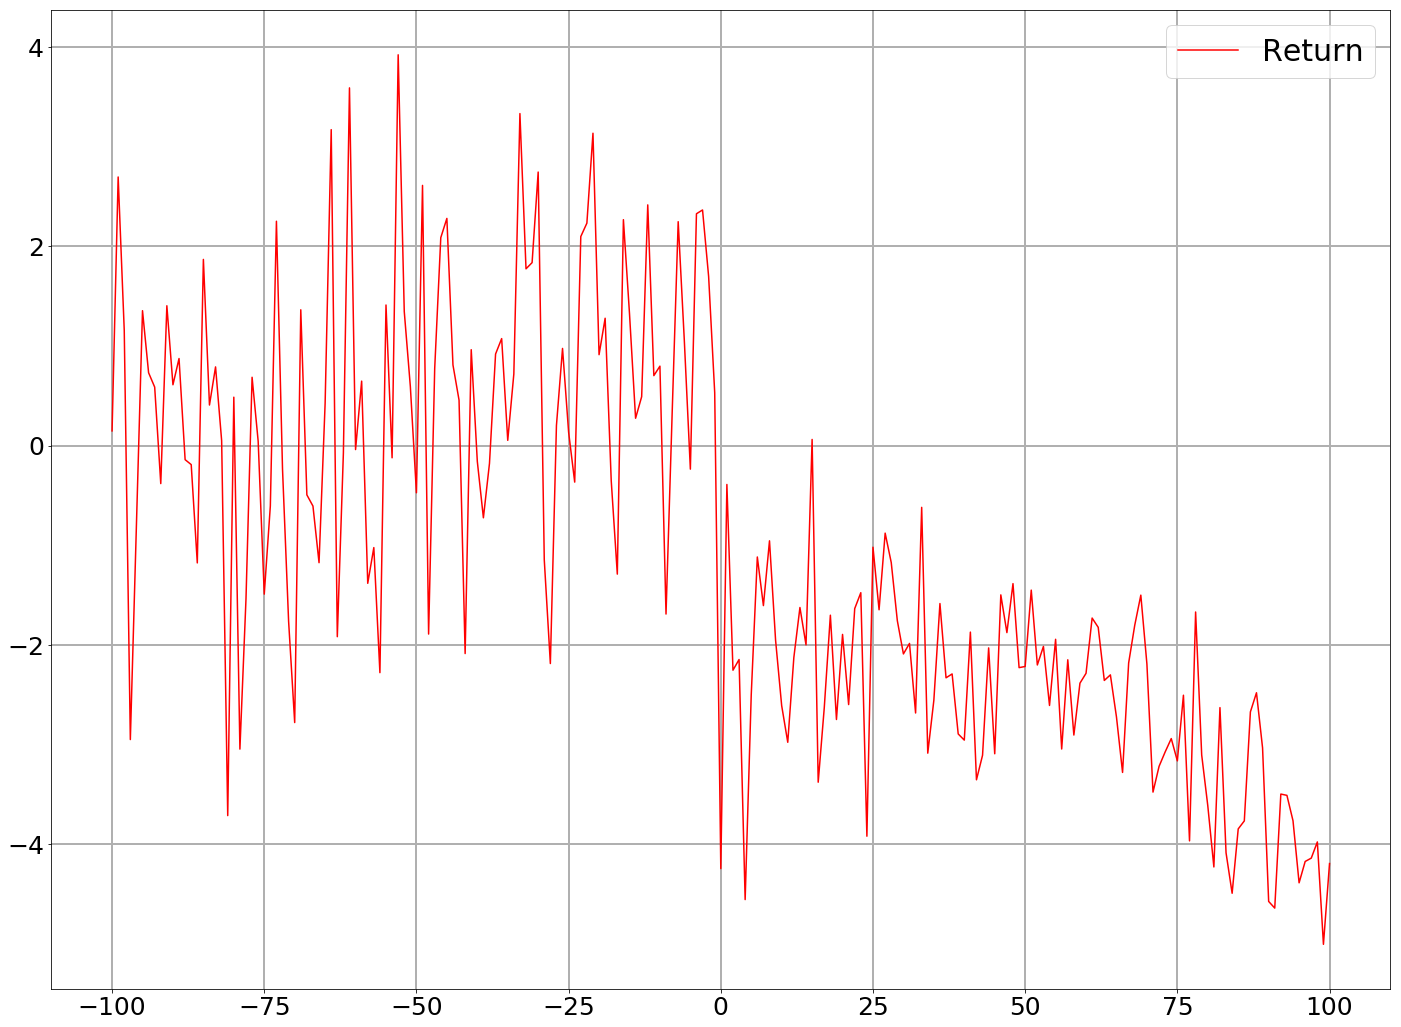
\includegraphics[width=\textwidth]{images/behaviour-up-100s-sell.png}
        \caption{Returns of sell orders 100 seconds}
        \label{fig:behvaiour-up-100s-sell}
    \end{subfigure}
    \caption{Returns of buy and sell orders executed within 10, 30, 60 and 100 seconds on data set II.}
    \label{fig:behvaiour-up}
\end{figure}

\section{Q-Learning without market variables}
The previous section provided knowledge about the possibilities of the agent when placing buy and sell orders using the reinforcement learning environment and with the underlying data set I and II.
The expected behaviour for each limit level has been observed under two significantly different market situations.
More precisely, it has been shown that during an upwards trend, market participants are willing to buy and sell shares for higher prices and contrarily, during a downwards trend for lower prices.
It has been observed that an agent would therefore indeed be able to place its orders accordingly in order to minimize the price to pay, respectively maximize the price for which to receive, the assets.

This section aims to reproduce the optimal achieved results shown in the previous section with the use of the Q-Learning agent as described in Chapter \ref{chap:setup} (Section \ref{setup:q-learning}).


\section{Deep Q-Network on execution}

\section{Deep Q-Network on market making}

\section{Deep Q-Network with event flow data}
